\chapter{Colorization}
\label{chapterlabel3}

Colourization is the process of adding plausible colours to monochrome images, it is a highly uncertain problem that does not have a unique solution. In the context of this master project, we are interested in anime-style sketch colourization, a few distinctive characteristics include:

\begin{itemize}
    \item Unlike grayscale image input, its input is a binary sketch image.
    \item Unlike realistic image colourization, the output is heavily style-oriented, has less well-defined details, and therefore comparably nondeterministic nature.
    \item Unlike many colourization types of research, the task of filling missing regions is not assessed. The full sketch image is provided without cropping.
    \item It is relatively difficult to find a dataset that contains a large number of high-quality pairs of sketch and colourized anime images, because artists often do not include them when uploading to the internet.
\end{itemize}


\section{Approaches \& Methods}
Anime-style sketch colourization is a sub-field in the image-to-image translation tasks. It is a difficult problem because there is an infinite number of ways to produce feasible results, therefore colour strokes are often given as additional input to hint the model to output in a certain style (user-guided colourization). There are many attempts to this problem and I will introduce them in the following paragraphs.

Traditional computer-assisted colourization uses an algorithmic approach. Typically, the user first crops the region that he/she wants to colour, then apply a colour scheme from a palette, and finally, the computer will run an algorithm to perform colourization. A popular approach is to minimize the difference between a pixel's colour and its weighted average of neighbouring pixels' colours.\cite{levinColorizationUsingOptimizationb} The intuitive is neighbouring pixels with similar intensity should have similar colours. This method generates high-quality results, but it is time-consuming because it requires detailed colour input and manual cropping. Follow-up research attempted to reduce the effort via learning-based methods, such as interpolation of user-drawn scribbles using boosting \cite{liScribbleBoostAddingClassification2008} or manifold learning \cite{chenManifoldPreservingEdit2012}; and determine the importance of image feature automatically using neural network \cite{endoDeepPropExtractingDeep2016}.


\begin{figure}
    \centering
    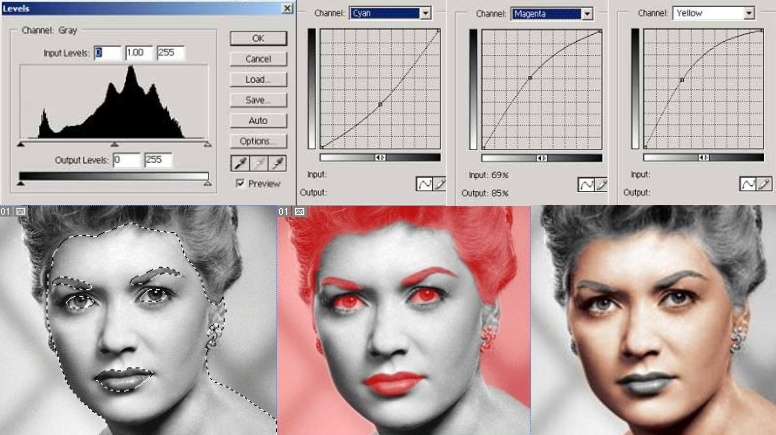
\includegraphics[width=0.75\textwidth]{images/colorization/computer_assisted_colorization.jpg}
    \caption{Example interface for traditional computer-assisted algorithmic colourization. The top shows an interface for selecting a colour; the bottom-left and bottom-middle show interfaces for selecting a region; and the bottom-right shows the resulting image.\cite{ColorizeBlackWhite}}
    \label{fig:computer_assisted_colorization}
\end{figure}

While these methods introduced remarkable improvements, image colourization remains a time-consuming task. In addition, traditional methods often make use of intensity information which does not present in anime sketches, which made them unsuitable. In recent years, machine learning-based methods started to gain popularity as the availability of computing resources increases. The milestone work of Pix2pix\cite{isolaImagetoImageTranslationConditional2018} demonstrated a simple yet general architecture for image-to-image translation task. It outperforms vanilla CNN by a large margin (see figure \ref{fig:colorization_cnn} for vanilla CNN outputs) However, directly apply Pix2pix model will result in artifacts such as \textit{color bleeding}\footnote{Color overflows boundaries defined by sketches.} and \textit{dirtiness}\footnote{Abrupt smoky color patches that are not defined by the sketches.}, they result in inconsistency and unpleasing colorization (see figure \ref{fig:colorization_pix2pix} for Pix2pix outputs). 

\begin{figure}
    \centering
    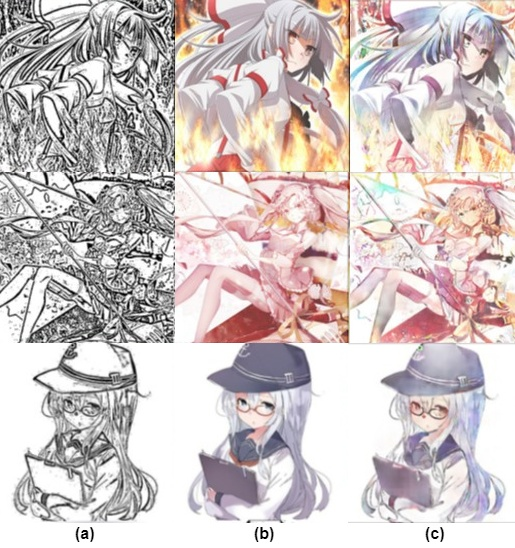
\includegraphics[width=0.75\textwidth]{images/colorization/cnn.jpg}
    \caption{Vanilla CNN output for anime sketch colourization. Column (a) is the input sketches; column (b) is the target image, and column (c) is the output image.\cite{fransOutlineColorizationTandem2017} We can see that the output suffers from a number of obvious issues, such as random fading and dirty colours, and obvious convolutional artefacts. It is far from visually pleasing.} 
    \label{fig:colorization_cnn}
\end{figure}

\begin{figure}
    \centering
    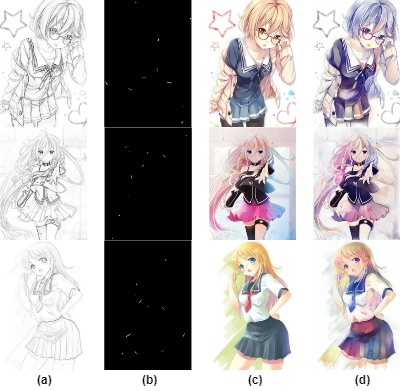
\includegraphics[width=0.85\textwidth]{images/colorization/pix2pix.jpg}
    \caption{Vanilla Pix2pix output for anime sketch colourization. Column (a) is the input sketches; column (b) is the colour hint; column (c) is the target image, and column (d) is the output image.\cite{steinsDeepLearningProject2022} The colouring is reasonable but suffers from artefacts such as colour bleeding and has a certain degree of dirtiness. For example, the colours are different on each stripe of the skirt. But we can also observe that the colour is more coherent than the vanilla CNN models as fewer convolution artefacts are produced.} 
    \label{fig:colorization_pix2pix}
\end{figure}

PetalicaPaint\cite{PetalicaPaint} used a doubly linked deep U-Net architecture to address the style inconsistency problem, by having a deeper network, the model is able to capture the general distribution and keep it consistent. However, its style varies on loss function hyper-parameters which means each model can only paint with one style (see figure \ref{fig:colorization_petalica}).

\begin{figure}
    \centering
    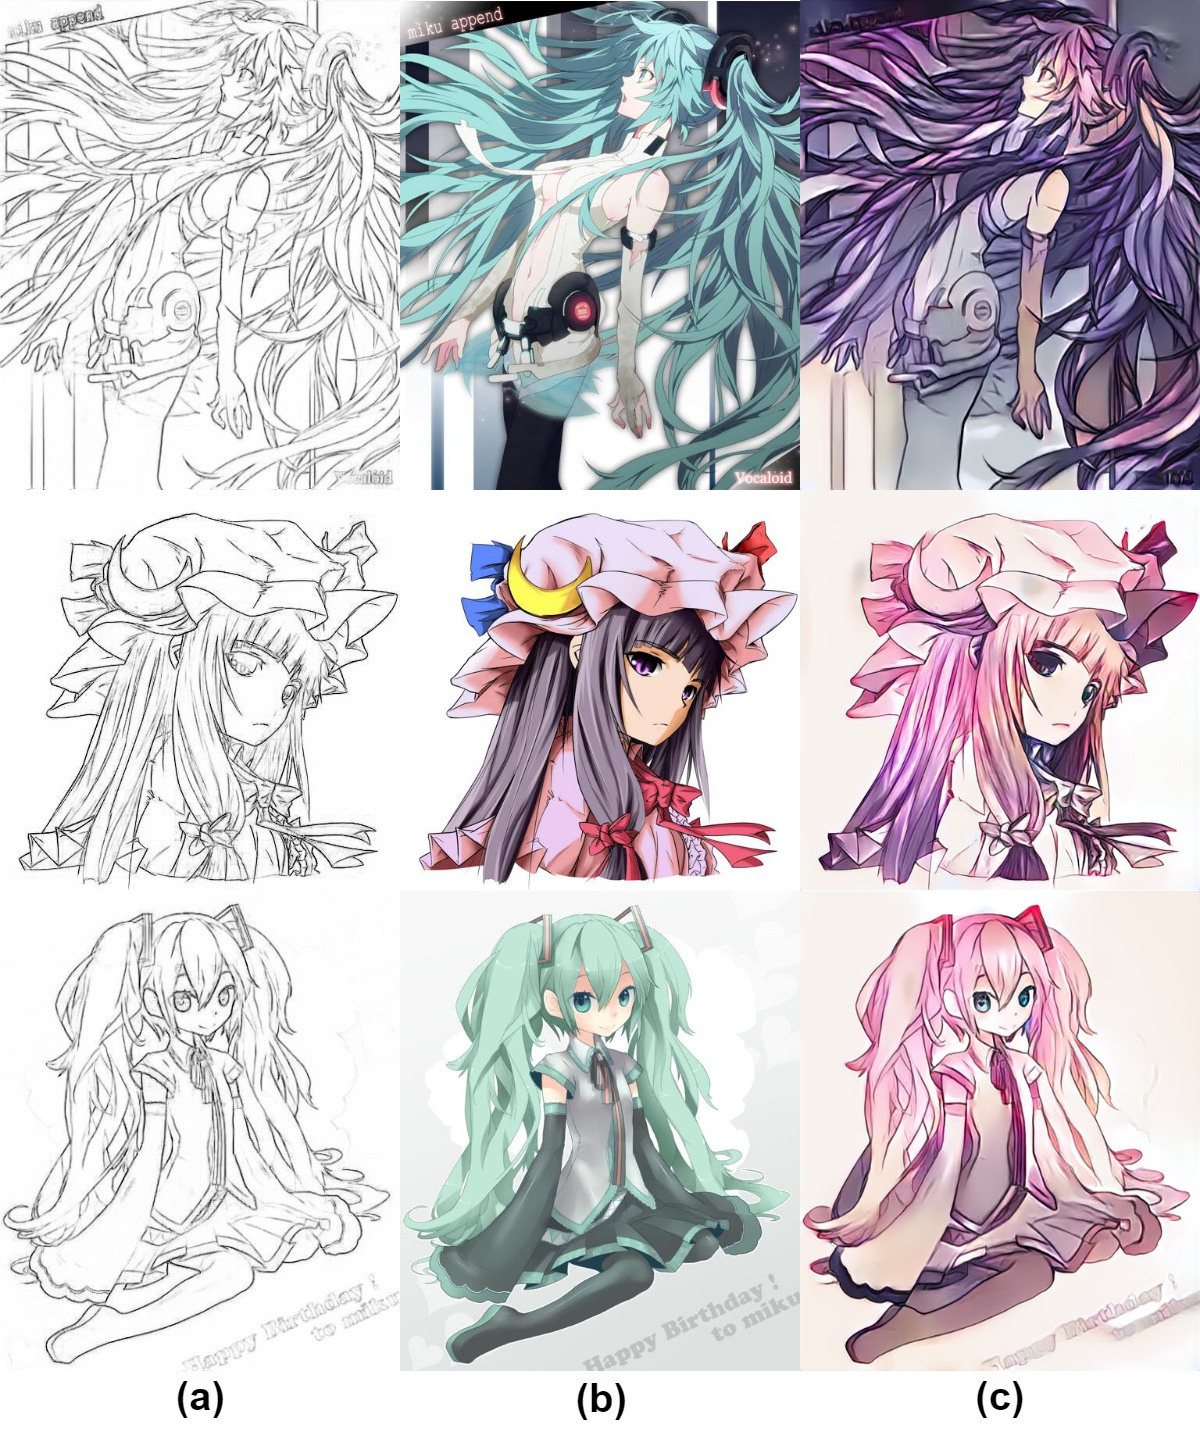
\includegraphics[width=0.75\textwidth]{images/colorization/petalica.jpg}
    \caption{Petalica Paint output for anime sketch colorization, painted with \textit{Canna\protect\footnotemark}  style. Column (a) is the input sketches; column (b) is the target image, and column (c) is the output image.\cite{steinsDeepLearningProject2022} The colouring showed consistency across the different regions with clean and plausible colouring with local shading, however, there is little artistic texture and global shading present in the coloured image.} 
    \label{fig:colorization_petalica}
\end{figure}

\footnotetext{The name of the style given to a particular model by the author.}

Although the result is much more pleasing, it is still not as vivid as most coloured images, the two most obvious features missing are artistic texture and global shading. Artistic texture allows the model to have slightly different styles in different regions of the image and global shading allows the model to draw sensible shadows and highlights. Fortunately, follow-up research showed that we can obtain artistic texture by using content loss and obtain global shading simply by increasing the receptive field of the U-Net block's decoders\cite{ciUserGuidedDeepAnime2018}. This is the AlacGAN model, which I will explain in detail below, sample output can be found in figure \ref{fig:colorization_alacgan}.

\begin{figure}
    \centering
    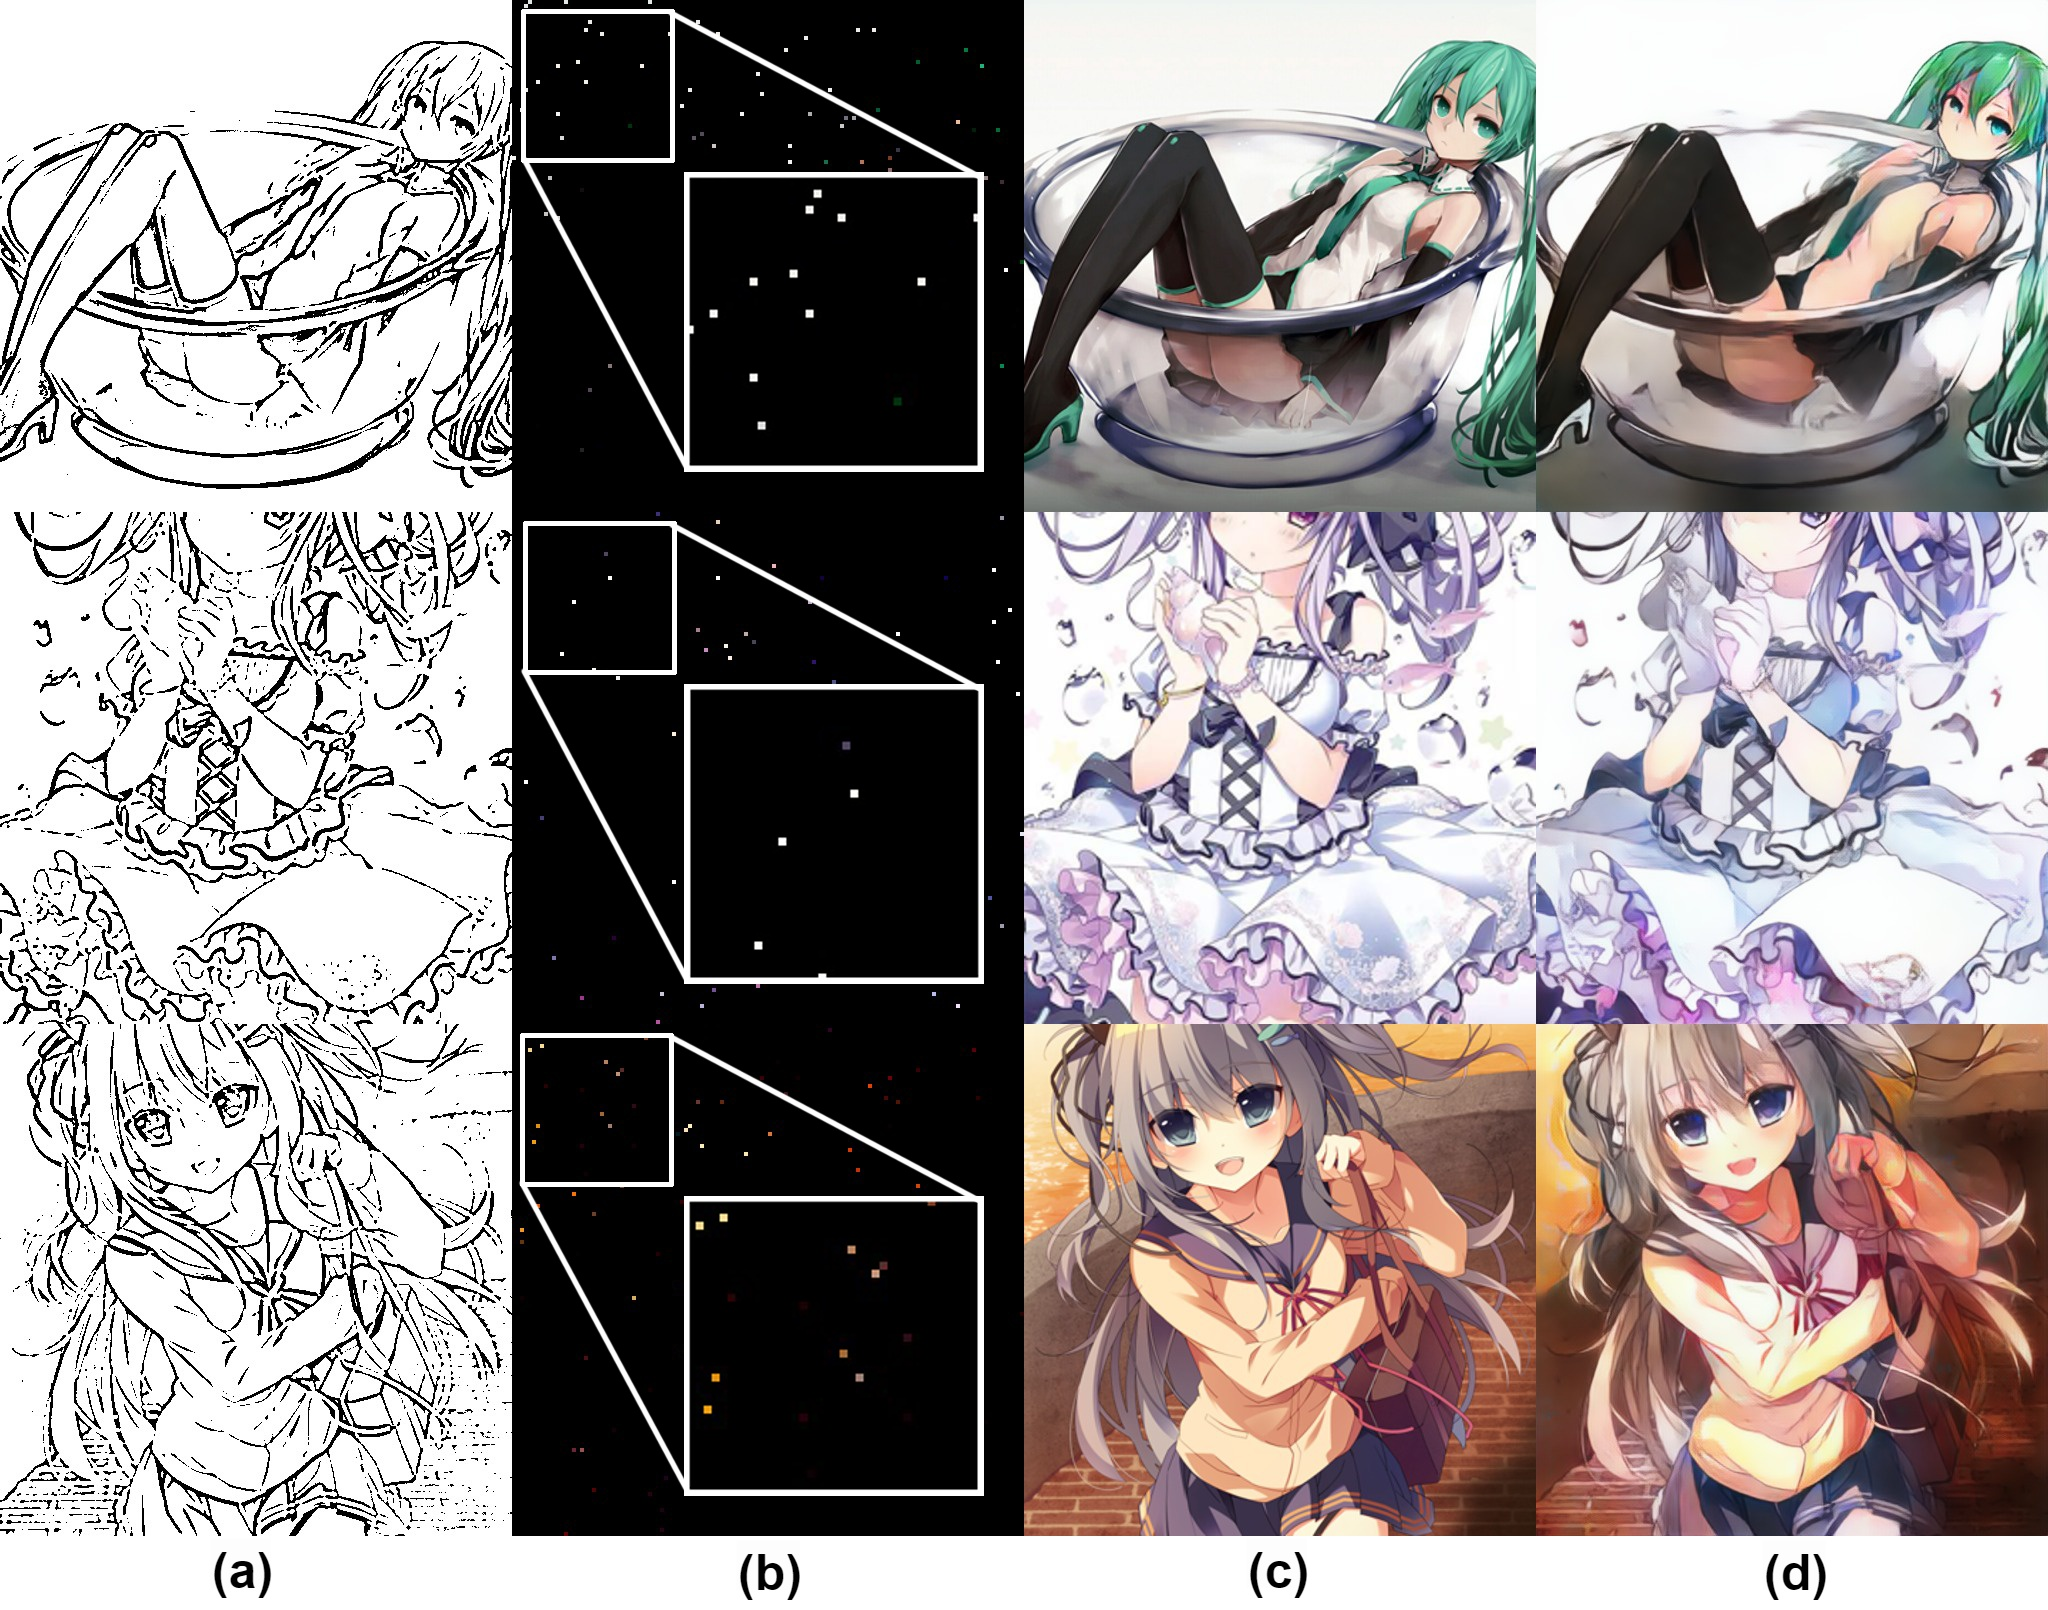
\includegraphics[width=0.85\textwidth]{images/colorization/alacgan.jpg}
    \caption{AlacGAN output for anime sketch colourization. Column (a) is the input sketches; column (b) is the colour hint, the white box enlarges a part of the hint for ease of viewing sample points; column (c) is the target image, and column (d) is the output image. We can observe that the presence of global shading and diverse artistic textures result in a much more vivid output.}
    \label{fig:colorization_alacgan}
    %\todo[inline]{enlarge part of the hint so that they are easier to see.}
\end{figure}

\section{Design \& Implementation}

\subsection{Dataset}
The input model is a binary anime sketch and the output is the colourized version of the sketch. It is difficult to find a large number of such pairs, most research generates sketches from coloured images. Real-world anime art contains a large variety of contents, and thus as a pre-trained model, our dataset should cover as many styles as possible to ensure its generality. Popular large illustration dataset such as Nico-opendata\cite{Undefineda} and Danbooru\cite{branwenDanbooru2021LargeScaleCrowdsourced2015} is not suitable because it contains many scribbles, resulting in hard-to-clean noise. Therefore I adopted the dataset from the original paper, which is crawled from the internet by the authors.

\subsection{Model}

% Tobias says he does not care about architecture 
% \begin{figure}
%     \centering
%     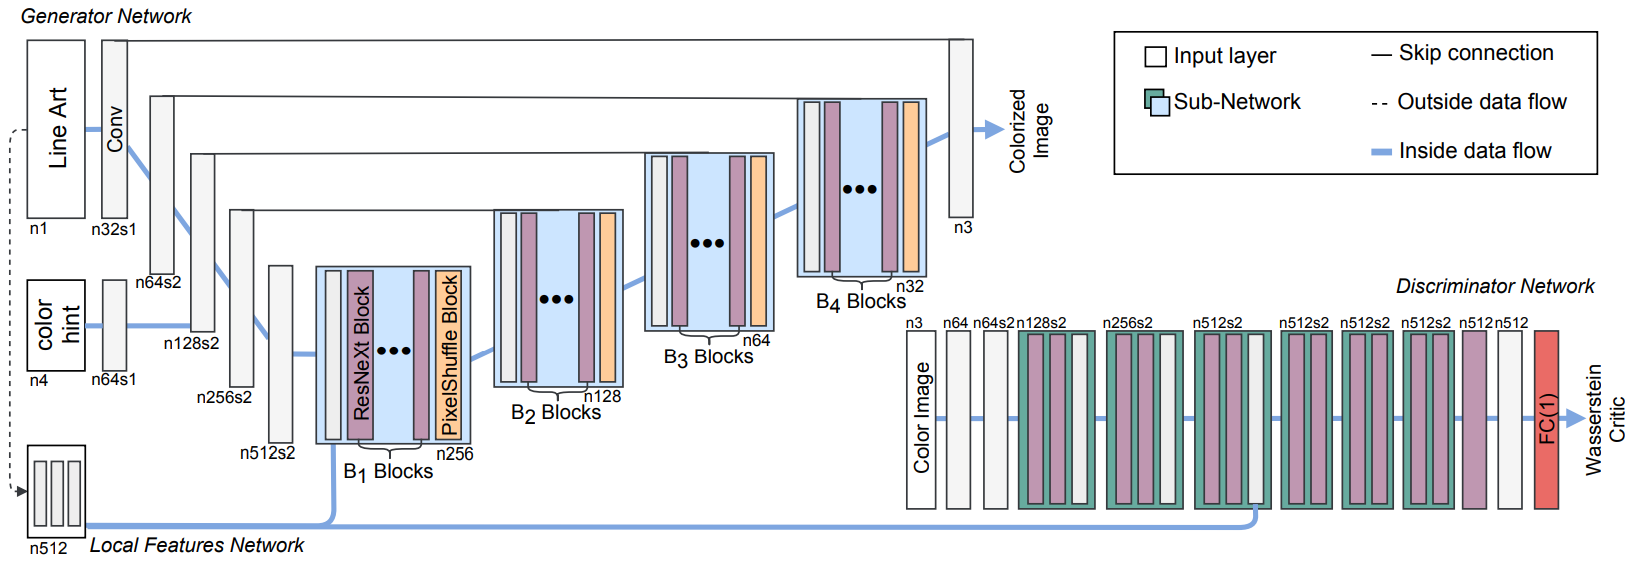
\includegraphics[width=1.0\textwidth]{images/colorization/alacgan_arch.png}
%     \caption{Architecture of Generator and Discriminator Network with the corresponding number of feature maps (n) and stride (s) indicated for each convolution block.} 
%     \label{fig:alacgan_arch}
% \end{figure}

The model follows a GAN architecture, including a generator $\mathcal{G}$ and a discriminator $\mathcal{D}$. The generator employs an U-Net\cite{ronnebergerUNetConvolutionalNetworks2015} architecture.
%Figure \ref{fig:alacgan_arch} shows the overall structure of the model.

The generator converts both the sketch and colour hint to the feature map and repeatedly convolutes and half-scales them until the features are the same size as the local feature network output. The local feature network is a pre-trained network that extracts features from the input sketch. Then both outputs are concatenated and repeatedly double-upscale using a sequential ResNeXt tunnel until the original dimension. The ResNeXt tunnel is a sequential stack of ResNeXt block\cite{xieAggregatedResidualTransformations2017a} with a pixel-shuffle block\cite{shiRealTimeSingleImage2016} appended at the end. It uses the ResNeXt block because it is more effective for increasing capacity compared to the vanilla resnet block without additional computational cost. Normalization layer is not used because it reduces flexibility for accurate colorization\cite{nahDeepMultiscaleConvolutional2018}.

The discriminator takes the concatenation of sketch features and coloured image as input, forming a cGAN\cite{mirzaConditionalGenerativeAdversarial2014} and employing an SRGAN\cite{ledigPhotoRealisticSingleImage2017} architecture without dilation as we do not need to upscale the image like the original paper does.

The local features are extracted from the sketch image using a pre-trained feature extraction network $\mathcal{F}1$. They contain both semantic and spatial information of the sketch. This helps to reduce overfitting on the synthetic sketches because human-drawn sketches can be very different from synthetic sketches, but the local feature network is pre-trained on human-drawn illustrations which will not affect by synthetic lines. Specifically, the $6^{th}$ convolution layer of the Illustration2Vec\cite{saitoIllustration2VecSemanticVector2015} network is used. It is pre-trained on 1,287,596 illustrations, including sketches and coloured images, predicting 1,539 labels.

The hint $H$ is randomly sampled pixels from the coloured image, the hint has the size 1/4 of the coloured image.

The second feature extractor $\mathcal{F}2$ is used to compute the content loss of the fake and real coloured image. It is the $4^{th}$ layer of the VGG16 network, pre-trained on ImageNet\cite{ImageNet}.

\begin{figure}
    \ centring
    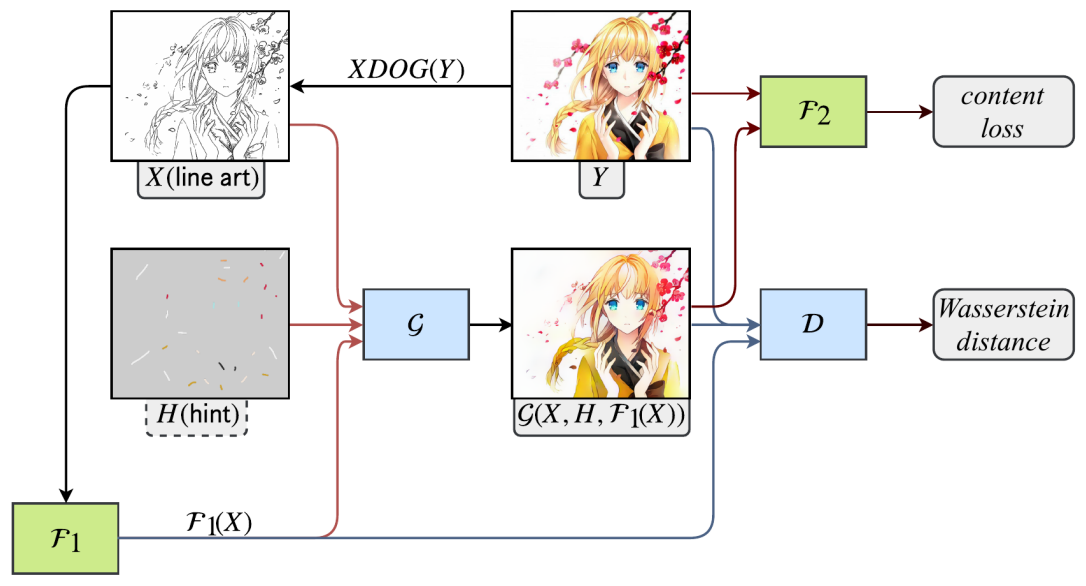
\includegraphics[width=0.75\textwidth]{images/colorization/alacgan_train.png}
    \caption{Overview of the training process of AlacGAN Network. $\mathcal{F}1$ and $\mathcal{F}2$ denotes two pre-trained feature extractors; $\mathcal{G}$ denotes generator and $\mathcal{D}$ denotes discriminator; $X$ denotes input sketch; $H$ denotes optional input colour hint; $Y$ denotes target coloured image and XDOG denotes the sketch generated from the coloured image.} 
    \label{fig:alacgan_train}
\end{figure}

\begin{figure}
    \centering
    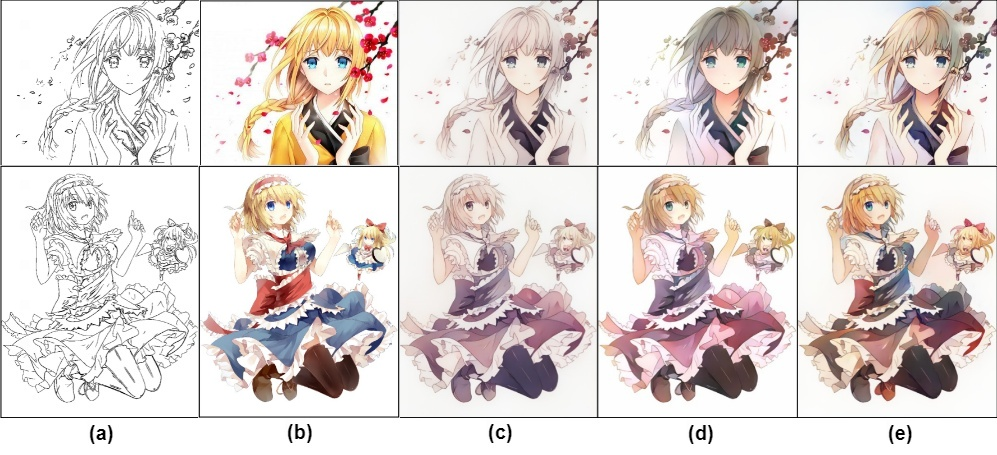
\includegraphics[width=1.0\textwidth]{images/colorization/alacgan_features.jpg}
    \caption{Comparison of different techniques used in AlacGAN. (a) denotes input sketch; (b) denotes the target output; (c) denotes output without adversarial loss; (d) denotes output without local feature network, and (e) denotes output when both exist. We can see that when an adversarial loss is missing, colour can be diluted. When the local features network is missing, global shading can be absent. When both techniques are used, the result looks much more vivid and closer to the target image.} 
    \label{fig:alacgan_features}
\end{figure}

\subsection{Preprocessing}
For each coloured image collected, I used the XDoG\cite{winnemollerXDoGEXtendedDifferenceofGaussians2012} algorithm to generate synthetic sketches that stimulate real sketch drawings. The settings are sigma = $0.3/0.4/0.5$; k sigma = $4.5$; epsilon = $0$; phi = $10\mathrm{e}9$; and gamma = $0.95$. Different sigmas are randomly chosen during training to stimulate different stroke thicknesses. During preprocessing, all three different sigmas images are generated beforehand to speed up training. All images are also cropped and resized to $512\times512$.
\todo[inline]{Add more details}

\subsection{Training}
I pre-trained with the following settings, similar to the original paper: batch size=8, epoch=500, optimizer=Adam, optimizer betas=(0.5, 0.999), learning rate=0.0001, scheduler=step, scheduler step size=400, scheduler gamma=0.1. The dataset contains 20k images, split for training and testing with a ratio of 9:1.

As for data augmentation, random resized crop, random jittering and random horizontal flip are applied to improve the model's generalization capability. After augmentation, images are also normalized with mean and variance of $0.5$ for more stabilized input.

\section{Analysis}
To ensure the pre-trained model indeed learnt a generalized colourization procedure. I conducted experiments on the intensity and colours of the colourization.

\subsection{Mask vs Maskless}
\begin{figure}
    \centering
    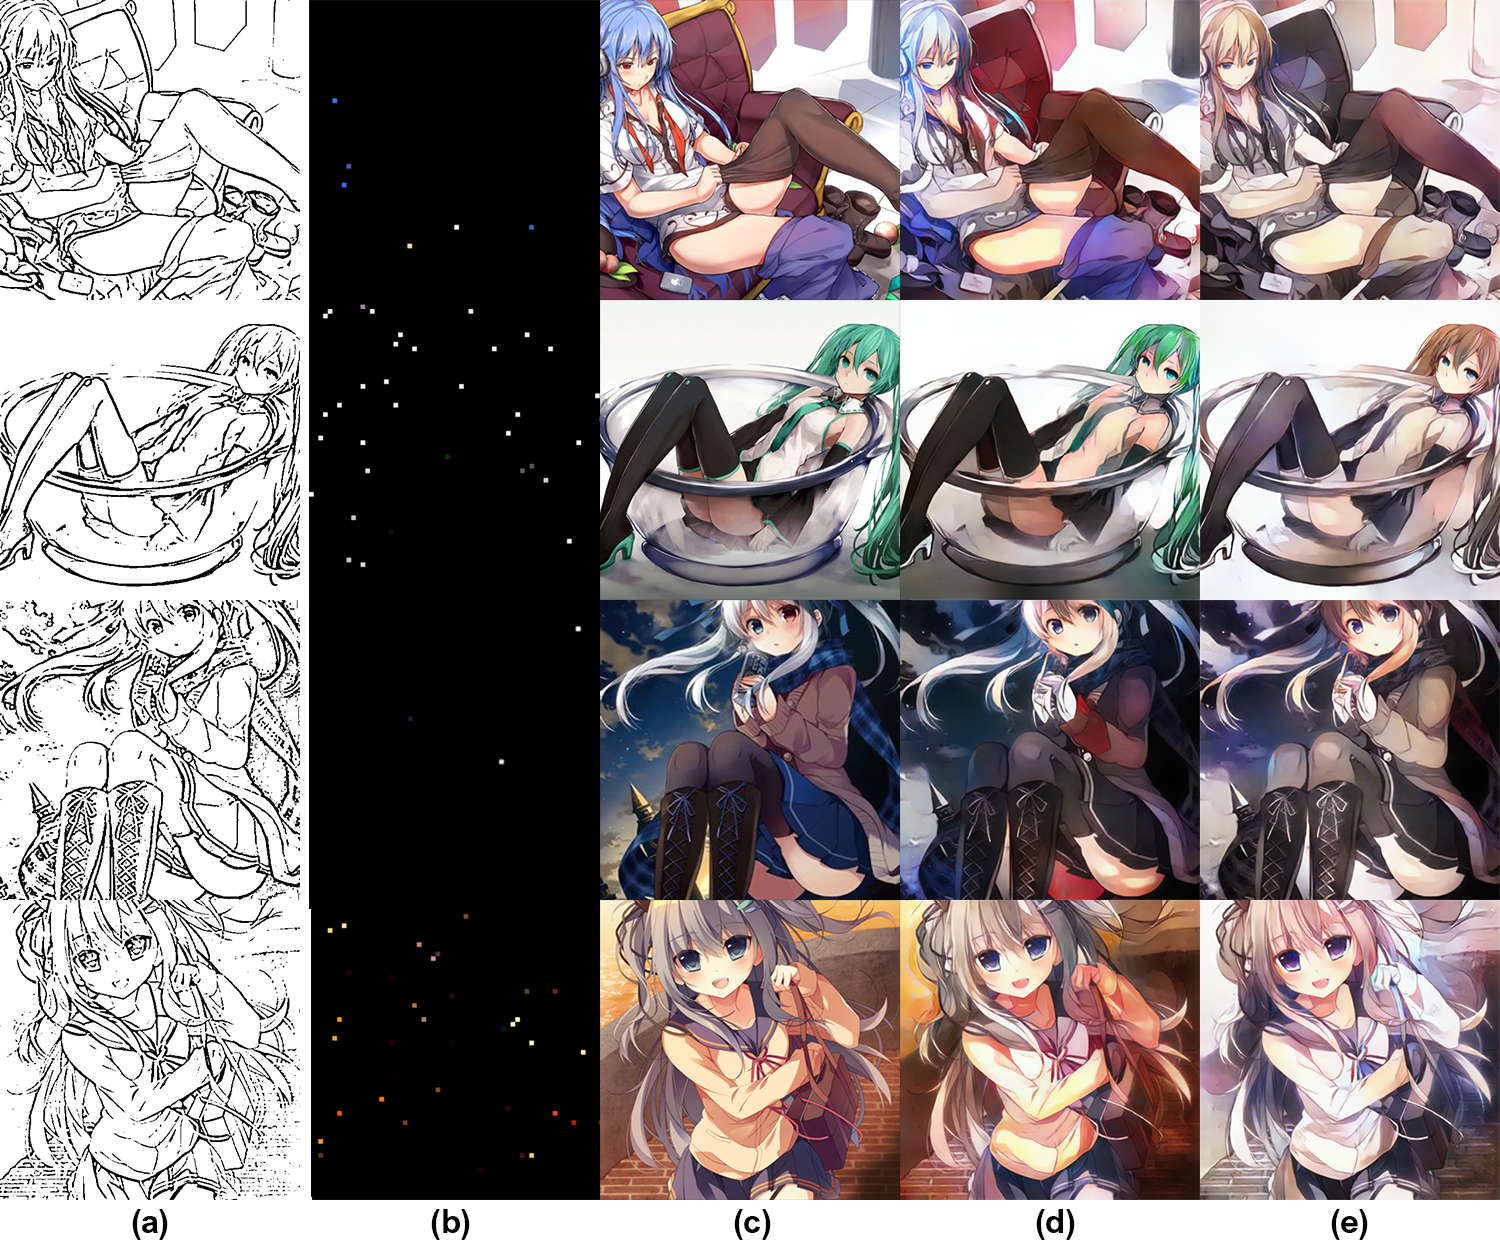
\includegraphics[width=1.0\textwidth]{images/colorization/mask_vs_maskless.png}
    \caption{Hint vs Hint-less colourization samples on the pre-trained model. Column (a) is the input sketch; column (b) is the input hint, which is randomly selected points from the target image, it only shows the top-left corner (25\%) of the input hint, so that it is easier to view some samples; column (c) is the  target image; column (d) is the colourized output with a hint; column (e) is the colourization output without a hint. We can observe that the hint-less output sticks to a coffee-colour-based palette, and the output with hint is able to produce a more diverse colourization output.}
    \label{fig:mask_vs_maskless}
\end{figure}

From figure \ref{fig:mask_vs_maskless}, we can see that the shading of the hint-less output suggests that light is coming from multiple directions. On the other hand, the output with a hint is able to identify the correct global shading. This means that by providing a colour hint, we implicitly suggest the light position in the scene.

\begin{figure}
    \centering
    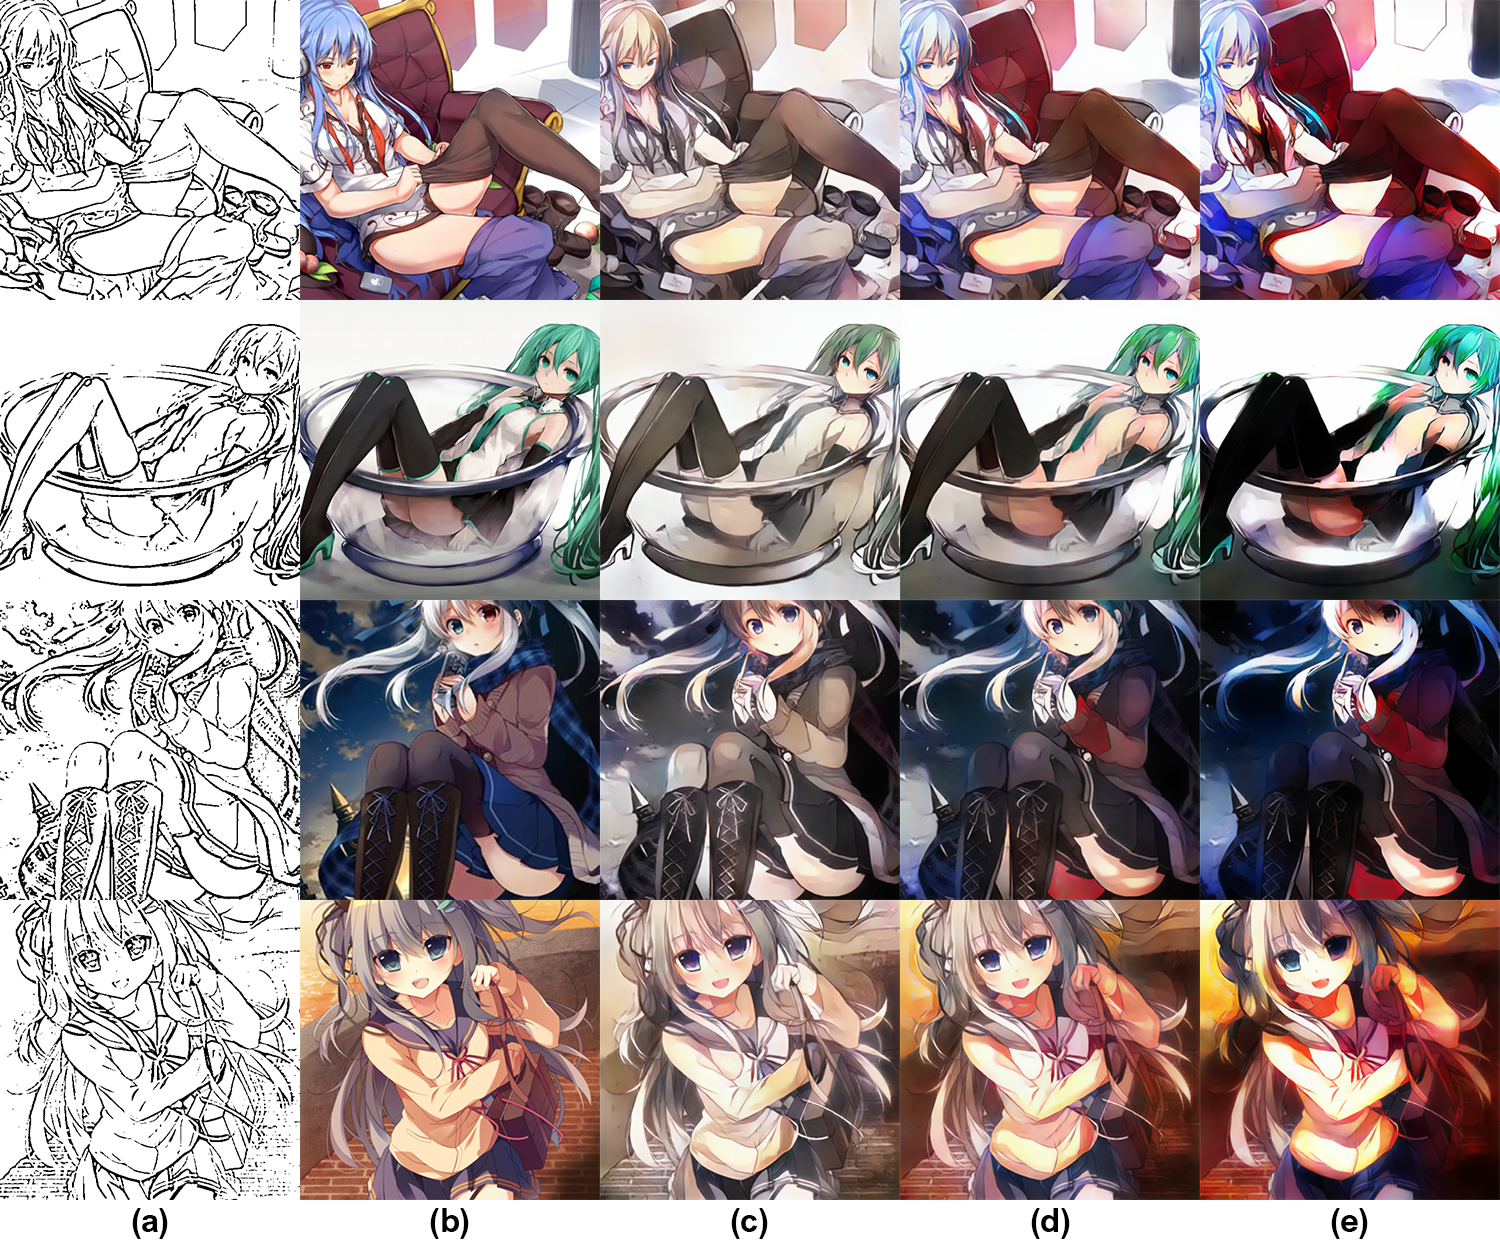
\includegraphics[width=1.0\textwidth]{images/colorization/lighter_vs_darker.png}
    \caption{Lighter vs Darker colourization samples on the pre-trained model. Column (a) is the input sketch; column (b) is the target image; column (c) is the colourized output with a hint multiplier of $0.25$; column (d) is the colourized output with a hint multiplier of $1.0$ (the normal output); column (e) is the colourized output with a hint multiplier of $3.0$. A \textit{hint multiplier} is a number that the input hint will be multiplied with before being passed into the model. We can observe that the colourized images are indeed getting darker as we darken the colour of the hint.}
    \label{fig:lighter_vs_darker}
\end{figure}

\begin{figure}
    \centering
    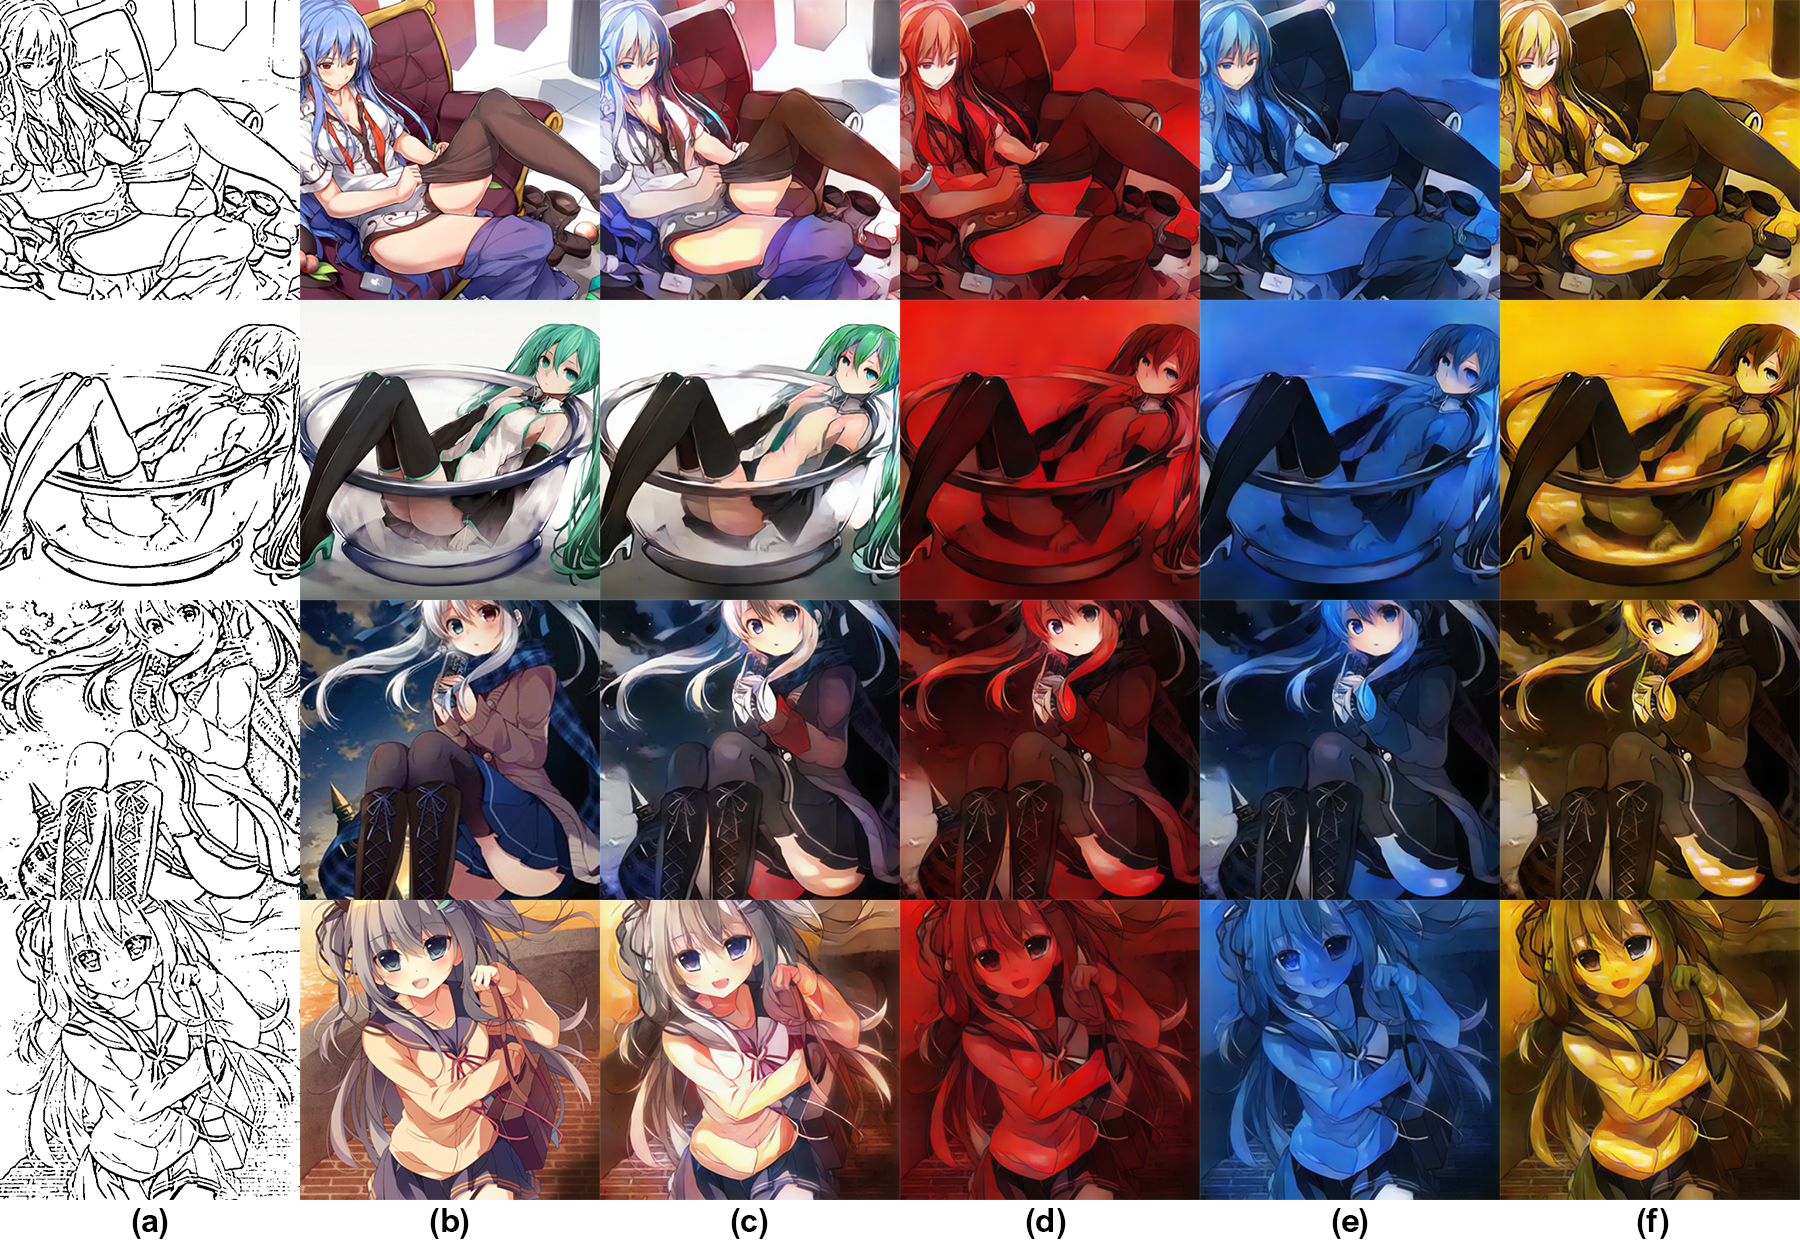
\includegraphics[width=1.0\textwidth]{images/colorization/RYB_comparison.png}
    \caption{Red-Blue-Yellow Colourization Comparison.}
    \label{fig:ryb_comparison}
\end{figure}



\section{Future Direction}
While AlacGAN can produce results with global shading and artistic texture, there is still room for improvement. First of all, although the model can generate coloured images according to colour hint input, there is little control over other aspects of the output. For example, the direction of light and colour tones. In the context of this master project, keeping the same object the same colour and styles constantly across hundreds of frames or even in another scene can be a challenging task.

As the most challenging task in this master project, the final AlacGAN model generates coloured images at 1 frame per second (FPS). It is expected to be the bottleneck of the whole pipeline. To improve the speed of the inference, we can attempt the following ideas:

\begin{itemize}
    \item \textbf{Knowledge distillation} The pre-trained local feature network can be useful at times but it can be computationally expensive and utilized at max capacity. We can introduce a smaller feature network and uses the pre-trained local feature network as the teacher to guide its learning. This processing is known as knowledge distillation (see appendix \ref{app:ml:kd}). This idea can be expanded to other parts of the network to further compress the model.
    \item \textbf{Domain specific tuning} The current model is pre-trained with thousands of online images, each of them coloured individually with detailed styling and artistic details. However, it is uncommon for 2D animation to achieve such a level of detail. By observing the frames from NoGhost, it is obvious that the most common colouring technique used is flat shading with little colour variation within the same enclosed region. Therefore, we could potentially reduce the receptive field of the ResNeXt convolution tunnels to achieve similar results.
\end{itemize}

